\section{Adversarial Machine Learning}\label{sec:adversarial-machine-learning}
Deep Learning algorithms have achieved the state-of-the-art performance in many tasks. 
However, the interpretability of deep neural networks is still unsatisfactory as they work as black boxes, which means it is difficult to get intuitions from what each neuron exactly has learned. 
One of the problems of the poor interpretability is evaluating the robustness of deep neural networks. 


Adversarial Machine Learning is a collection of techniques to train neural networks on how to spot intentionally misleading data or behaviors. 
This differs from the standard classification problem in machine learning, since the goal is not just to spot “bad” inputs, but preemptively locate vulnerabilities and craft more flexible learning algorithms.

The objective of an adversary
could be to attempt to manipulate either the data collection or
the data processing in order to corrupt the target model, thus
tampering the original output. 

Unlike traditional cybersecurity
attacks, these weaknesses are not due to mistakes made by programmers or users. They are
just shortcomings of the current state-of-the-art
methods. Put more bluntly, the algorithms that
cause AI systems to work so well are imperfect,
and their systematic limitations create opportunities for adversaries to attack. At least for the foreseeable future, this is just
a fact of mathematical life \cite{Comiter2019AttackingAI}.

Two main types of AI attacks can be defined according to the time at which the attack happens \cite{journals/corr/abs-1810-00069}:
\begin{itemize}
    \item \textbf{Adversarial Attacks (Evasion)}: this is the most common type of attack in
    the adversarial setting. The adversary tries to evade the system by adjusting malicious samples during testing phase. This
    setting does not assume any influence over the training data.
    In Figure \ref{fig:2_2_evasion} is depicted how adding an imperceptible and carefully constructed noise to the input originally regognized as “panda” with 57.7\% confidence, we can change
    the classification output given by the same neural network toward another target (in the example “gibbon” with 99.3\% confidence).
    \item \textbf{Data Poisoning Attacks}: This type of attack, known as contamination of the training data, is carried out at training phase of
    the machine learning model. An adversary tries to inject
    skilfully crafted samples to poison the system in order to
    compromise the entire learning process. The Figure \ref{fig:2_2_data_poisoning} shows as in normal machine learning (left), the learning algorithm extracts
    patterns from a dataset, and the “learned” knowledge is stored in the machine
    learning model---the brain of the system. In a poisoning attack (right), the
    attacker changes the training data to poison the learned model. 
\end{itemize}

\begin{figure}[H]
    \begin{subfigure}{0.45\textwidth}
      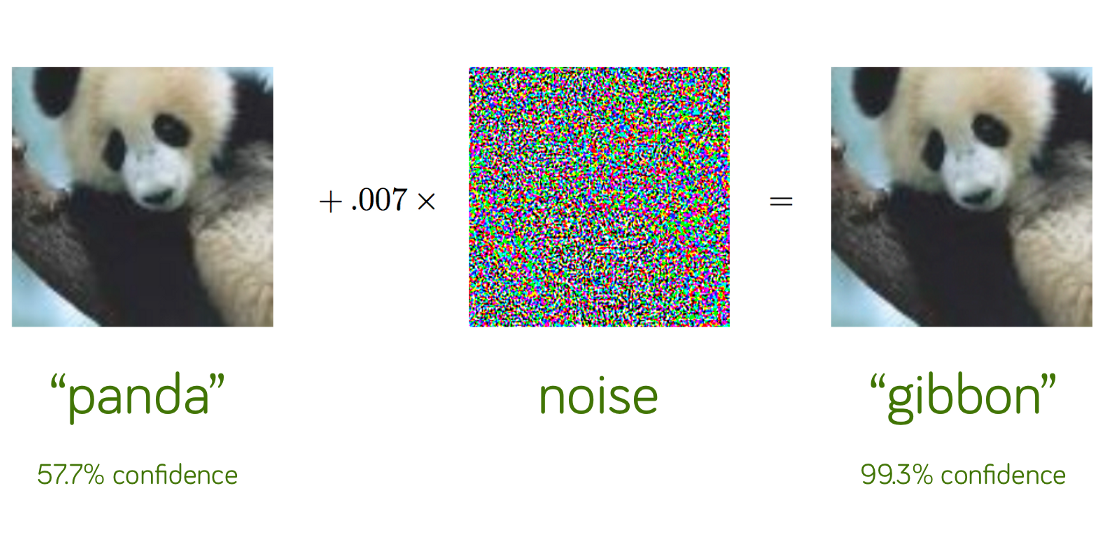
\includegraphics[width=\linewidth]{images/2_2_evasion.png}
      \caption{Evasion attack on image classification \cite{szegedy2013intriguing}} \label{fig:2_2_evasion}
    \end{subfigure}%
    \hspace*{\fill}   % maximize separation between the subfigures
    \begin{subfigure}{0.45\textwidth}
      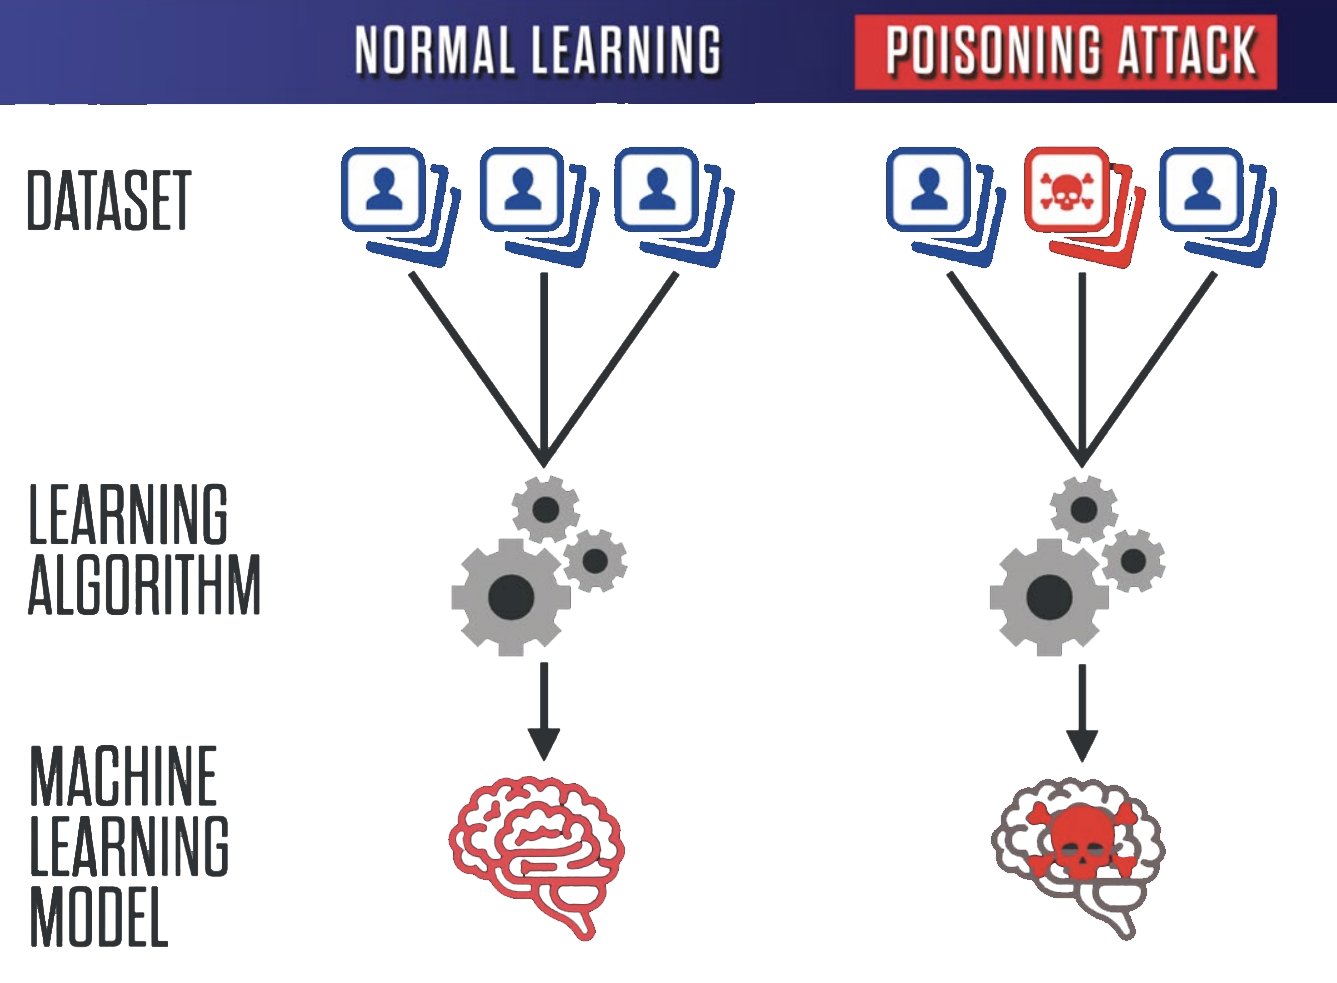
\includegraphics[width=\linewidth]{images/2_2_data_poisoning.png}
      \caption{Poisoning attack on training data \cite{Comiter2019AttackingAI}} \label{fig:2_2_data_poisoning}
    \end{subfigure}
  \caption{Examples of Artificial Intelligence Attacks} \label{fig:2_2_adversarial_attacks}
  \end{figure}

In this thesis, we will focus on the first type of attack, the Adversarial Attacks.
Over past few years, researchers \cite{goodfellow2014explaining, szegedy2013intriguing} used small unperceivable perturbations to evaluate the robustness of deep neural networks and found that they are not robust to these perturbations. 

%**************************************************************
\subsection{Adversarial examples}\label{subsec:adversarial-attacks}

Szegedy et al. \cite{szegedy2013intriguing} first evaluated the state-of-the-art deep neural networks used for image classification with small generated perturbations on the input images.
They found that the image classifiers were fooled with high probability, but human judgment is not affected. The perturbed image pixels were named \emph{adversarial examples} and this notation is later used to denote all kinds of perturbed samples in a general manner.
Formally, adversarial example $x^\prime$ is an example created via worst-case perturbation of the input to a deep learning model. An ideal deep neural network would still assign correct class $y$ (in the case of classification task) to $x^\prime$, 
while a victim deep neural network would have high confidence on wrong prediction of $x^\prime$. $x^\prime$ can be formalized as:
\begin{equation}
    \begin{array}{l}
    x^\prime = x + \eta, \quad f(x)=y, \quad x \in X,\\
    f(x^\prime) \neq y, \\
    \text{or} \quad f(x^\prime) = y^\prime, \quad y \neq y^\prime
    \end{array}
\end{equation}
where $\eta$ is the worst-case perturbation. The goal of the adversarial attack can be deviating the label to incorrect one ($f(x^\prime) \neq y$) or specified one ($f(x^\prime) = y^\prime$) \cite{journals/tist/ZhangSAL20}.

%**************************************************************
\subsection[Paradigm shift]{Paradigm shift: from CV to NLP}\label{subsec:paradigm-shift}
Adversarial examples were first proposed for attacking DNNs for object recognition in the \acrfull{cv} community.

%**************************************************************
\subsection{Taxonomy of textual adversarial attacks}\label{subsec:taxonomy-textual-adversarial-attacks}

%from https://arxiv.org/pdf/1810.00069.pdf

Adversarial attacks at the testing time do not tamper with the targeted model but rather forces it to produce incorrect outputs. The effectiveness of such attacks
is determined mainly by the amount of information available to the adversary about the model.
Testing phase attacks can be broadly classified into either White-Box or Black-Box attacks. Before
discussing these attacks, we provide a formal definition of a training procedure for a machine
learning model.
Let us consider a target machine learning model f is trained over input pair (X,y) from the
data distribution µ with a randomized training procedure train having randomness r (e.g., random
weight initialization, dropout, etc.). The model parameters θ are learned after the training procedure.
More formally, we can write:
θ ← train(f ,X,y,r)
Now, let us understand the capabilities of the white-box and black-box adversaries with respect
to this definition. An overview of the different threat models have been shown in Figure. 4
White-Box Attacks. In white-box attack on a machine learning model, an adversary has total
knowledge about the model (f ) used for classification (e.g., type of neural network along with

%**************************************************************
\subsection{Adversarial attack methods from literature}\label{subsec:aam-from-literature}

%--------------------------------------------------------------
\subsubsection{TextFooler}\label{subsubsec:textfooler}

%--------------------------------------------------------------
\subsubsection{BERT-based attacks}\label{subsubsec:bert-based-attacks}